\section{Grænseværdier og kontinuitet}
\begin{enumerate}
	\item Svarene er: $\lim_{x\to 1}f(x)=5$ og $f(1)=6$, hvorfor $f$ er ikke kontinuert.
	
	
	\item Svarene er: $\lim_{x\to 2}f(x)=7$ så $f$ er kontinuert da $ f(2)=7 $.

	
	
	\item Svarene er:
	\begin{align*}
	9,&& \ -1,&&\ -4,&& \frac{-2}{3}
	\end{align*}
	


	
	
	\item Grænsen eksisterer og er lig $1$ fra både højre og venstre.
	
	\item Svarene er: $f(1)=2$ samt at $f$ er ikke kontinuert i $1$ da $\lim_{x\to 1^+}f(x)=3$ og $\lim_{x\to 1^-}f(x)=1$.
	
	
	\item Svarene er: $a=5$ og $b=3$.
	
	\item\label{it:lim2ans} Svarene er: $ f(0) =0$, $ \lim_{x\to 0^+}f(x)=1 $ og $\lim_{x\to 0^-}f(x)=-1$. Funktionen $f$ er kontinuert i alle punkter undtagen $0$.
	
	\item Svarene er:
	\begin{align*}
	0,&& -6
	\end{align*}
	
	\item Svarene er: 
	\begin{enumerate}
		\item $ (f+g)(0)=0$, $ \lim_{x\to 0^+}(f+g)(x)=0 $ og $\lim_{x\to 0^-}(f+g)(x)=0$. Funktionen $(f+g)$ er kontinuert i alle punkter.
		\item $ (fg)(0) =0$, $ \lim_{x\to 0^+}(fg)(x) =-1$ og $\lim_{x\to 0^-}(fg)(x)=-1$. Funktionen $(fg)$ er kontinuert i alle punkter undtagen $0$.
	\end{enumerate}
	
	\item Svarene er:
	\begin{enumerate}
		\item $a=\frac{\sqrt{2}}{2}$.
		\item Da $\lim_{x\to 0}=2$ og $f(0)=1$ er funktionen ikke kontinuert når $a=0$.
	\end{enumerate}

	\item Svarene er:
	\begin{align*}
	0,&& 6e^4,&&  \ln \frac{1}{2}.
	\end{align*}
	
	\item\label{it:lim1ans} Svarene kan være:
	\begin{enumerate}
		\item Arealet af $\Delta ABD$ er givet ved $\frac{1}{2}\sin(x)$ da grundlinjen i trekanten er $1$. Arealet af enhedcirklen er $\pi$ så da det grå cirkeludsnit udgør $ \frac{x}{2\pi} $ af hele cirklen må dets areal være $ \pi\frac{x}{2\pi}=\frac{x}{2} $. Arealet af $\Delta ACD$ er givet ved $\frac{1}{2}\tan x$ da grundlinjen i cirklen er $1$. Det er klart at $\Delta ADB$ har areal mindre end det grå cirkeludsnit som så har areal mindre end $\Delta ACD$. Dette giver den ønskede ulighed
		\begin{align*}
		\frac{1}{2}\sin x\leq \frac{1}{2}x\leq \frac{1}{2}\tan x.
		\end{align*}
		
		\item Ved at gange uligheden med $2$ og dividere med $\sin x$ får vi
		\begin{align}\label{eq:1}
		1\leq \frac{x}{\sin x}\leq \frac{1}{\cos x}.
		\end{align}
		Bemærk at vi har brugt at $\tan x=\frac{\sin x}{\cos x}$. Hvis vi ganger den første ulighed i~\eqref{eq:1} igennem med $\frac{\sin x}{x}$ får vi at
		\begin{align}\label{eq:2}
		\frac{\sin x}{x}\leq 1.
		\end{align}
		Ganger vi den anden ulighed i~\eqref{eq:1} igennem med $\frac{\sin(x)\cos(x)}{x}$ får vi at 
		\begin{align}\label{eq:3}
		\cos x\leq \frac{\sin x}{x}.
		\end{align}
		Kombinerer vi~\eqref{eq:2} og~\eqref{eq:3} får vi den ønskede ulighed
		\begin{align}\label{eq:4}
		\cos(x)\leq \frac{\sin x}{x}\leq 1.
		\end{align}

		
		\item Fra~\eqref{eq:4} ses at $ \frac{\sin x}{x} $ ligger mellem $\cos x$ og $1$. Når $x$ går mod $0$ går $\cos x$ mod $1$ og da uligheden gælder for alle $x$ tæt på nul må $\frac{\sin x}{x}$ nødvendigvis også gå mod $1$. Man kan se det som at $\frac{\sin x}{x}$ bliver klemt sammen af $\cos x$ og $1$ omkring punktet $x=0$ (se evt. Figur~\ref{fig:trig5}).
	\end{enumerate}

	\begin{figure}
	\centering
	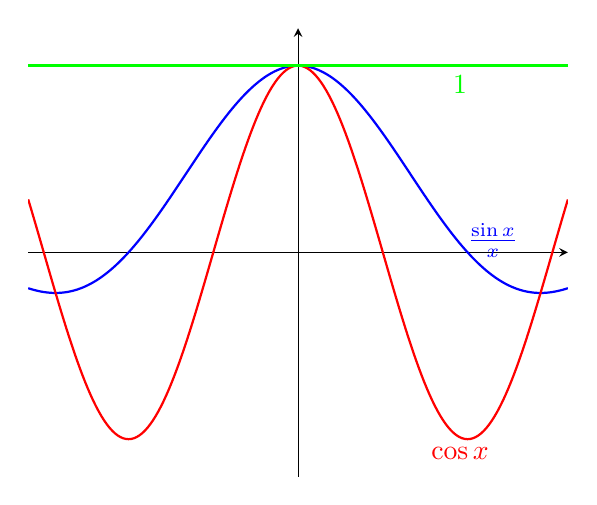
\begin{tikzpicture}
	\begin{axis}[xmin=-5,xmax=5,ymin=-1.2,ymax=1.2,axis x line=center,
	axis y line=center,ticks=none]
	\addplot[blue,thick,samples=200] {sin(deg(x))/x} node[pos=0.8,above,right] {$\frac{\sin x}{x}$};
	\addplot[red,thick,samples=200] {cos(deg(x))} node[pos=0.8,below] {$\cos x$};
		\addplot[green,thick,samples=200] {1}node[pos=0.8,below] {$1$};
	\end{axis}
	\end{tikzpicture}
	\caption{Funktionen $ \frac{\sin x}{x} $ ``klemmes'' af $1$ og $\cos x$.}
	\label{fig:trig5}
\end{figure}

	
%	\begin{figure}
%		\centering
%		\begin{tikzpicture}
%		\begin{axis}[xmin=-0.2,xmax=1,ymin=-0.2,ymax=1.2,axis x line=center,
%		axis y line=center, axis equal]
%				\pgfmathsetmacro\foo{sqrt(2)/2}
%		\draw[fill=gray!40] (axis cs:0,0)--(axis cs:1,0)--(axis cs:\foo,\foo);		
%		\draw[fill=gray!40] (axis cs:1,0)  arc[start angle=0, end angle=45,radius={transformdirectionx(1)}];
%
%		\addplot[blue,domain=0:2*pi,thick, samples=100] ({cos(deg(x))},{sin(deg(x))});
%		\addplot[domain=0:1,thick] {x};
%		\addplot[domain=0:pi/4,thick,samples=100] ({0.2*cos(deg(x))},{0.2*sin(deg(x))}) node[label={[label distance=2pt]0:\small$x$},pos=0.5] {};
%		\addplot[dotted,thick] coordinates {({sqrt(2)/2}, {sqrt(2)/2}) ({sqrt(2)/2}, 0)};
%		\addplot[domain=sqrt(2)/2:1,thick] {{-x*sqrt(2)/(2-sqrt(2))+sqrt(2)/(2-sqrt(2))}};
%		\addplot[thick] coordinates {(1,1) (1,0) };
%		
%		\node[fill, circle, inner sep=1pt] at (axis cs:0,0) [label=above left: $A$]{};
%		\node[fill, circle, inner sep=1pt] at (axis cs:\foo,\foo) [label=above: $B$]{};
%		\node[fill, circle, inner sep=1pt] at (axis cs:1,1) [label=above: $C$]{};
%		\node[fill, circle, inner sep=1pt] at (axis cs:1,0) [label=above right: $D$]{};
%		\end{axis}
%		\end{tikzpicture}
%		\caption{Opgave~\ref{it:lim1}}
%		\label{fig:lim1}
%	\end{figure}

	\item\label{it:lim3ans} Hvis vi benytter os af hintet får vi
	\begin{align*}
	\lim_{x\to 0}\frac{\cos(x)-1}{x}=\Big(\lim_{x\to 0}\frac{\sin x}{x}\Big)\Big(\lim_{x\to 0}\frac{\sin x}{1+\cos x}\Big)=\frac{\sin 0}{1+\cos 0}=0.
	\end{align*}
	
	\item Hvis vi trækker $1$ fra på alle sider af ulighederne i~\eqref{eq:4} og dividerer med $x\neq 0$ får vi at 
	\begin{align*}
	\cos(x)-1\leq \frac{\sin x}{x}-1\leq 0\quad\Leftrightarrow \quad \frac{\cos(x)-1}{x}\leq \frac{\sin(x)-x}{x^2}\leq 0.
	\end{align*}
	 Vi ved fra Opgave~\ref{it:lim3} at 
	 \begin{align*}
	\lim_{x\to 0}\frac{\cos x-1}{x}=0,
 	\end{align*}
	så igen giver et klemmeargument at $\lim_{x\to 0}\frac{\sin(x)-x}{x^2}=0$ (se evt. Figur~\ref{fig:trig6}).
	\begin{figure}
	\centering
	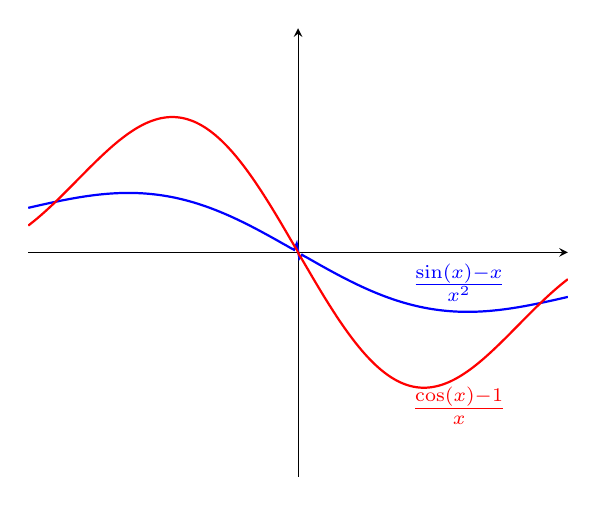
\begin{tikzpicture}
	\begin{axis}[xmin=-5,xmax=5,ymin=-1.2,ymax=1.2,axis x line=center,
	axis y line=center,ticks=none]
	\addplot[blue,thick,samples=200] {(sin(deg(x))-x)/x^2} node[pos=0.8,above] {$\frac{\sin(x)-x}{x^2}$};
	\addplot[red,thick,samples=200] {(cos(deg(x))-1)/x } node[pos=0.8,below] {$\frac{\cos(x)-1}{x}$};
	\end{axis}
	\end{tikzpicture}
	\caption{Funktionen $ \frac{\sin(x)-x}{x^2} $ ``klemmes'' af $0$ og $\frac{\cos x-1}{x}$.}
	\label{fig:trig6}
	\end{figure}

	
	
	\item\label{it:lim5ans} Hvis vi benytter os af hintet får vi	
	\begin{align*}
	\lim_{x\to 0}\frac{\cos x-1}{x^2}=\Big(\lim_{x\to 0}\frac{\sin x}{x}\Big)^2\Big(\lim_{x\to 0}\frac{1}{1+\cos x}\Big)=\frac{1}{1+\cos 0}=\frac{1}{2}.
	\end{align*}
\end{enumerate}